\begin{figure}[!htbp]\centering
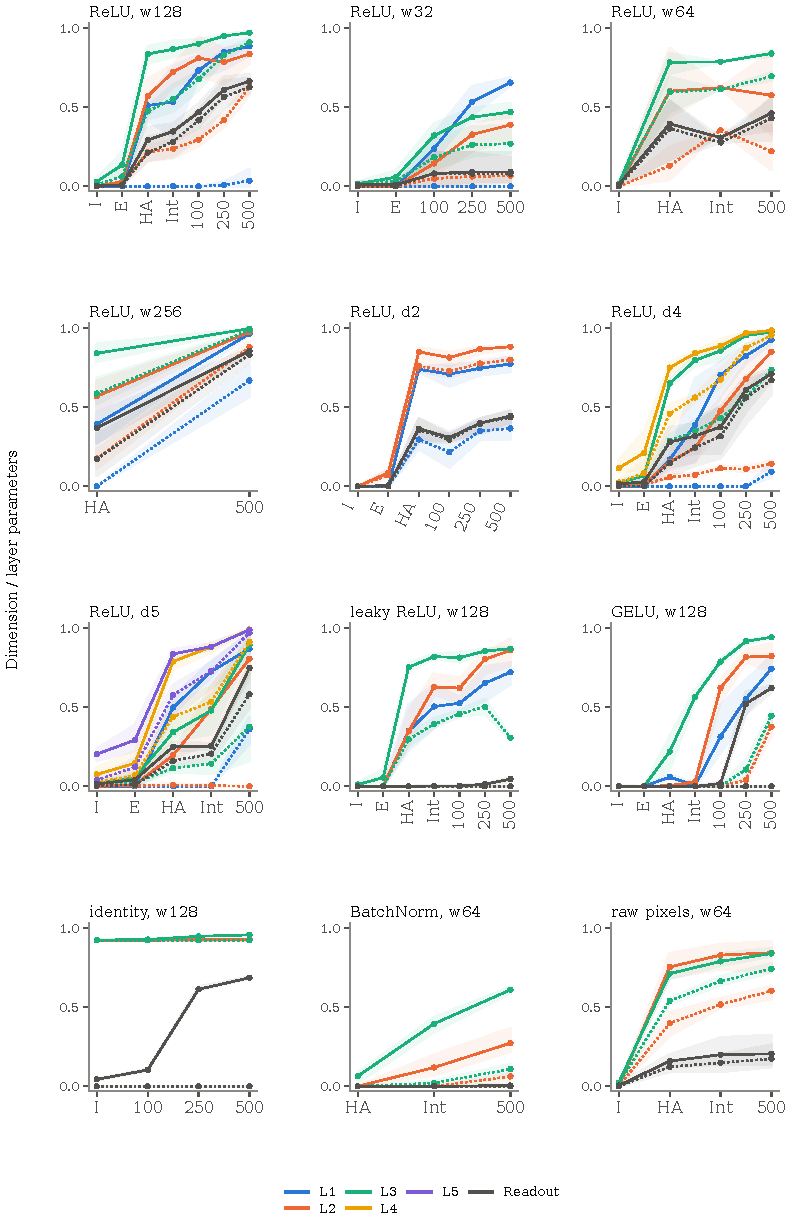
\includegraphics[width=4.754in]{compact_tails_part1.pdf}
\caption{Approximate atomic dimensions for models measured at multiple training stages, with all measured layers shown. MNIST is used unless labeled SVHN; layer numbers refer to hidden layers or convolutional layers. Solid curves count singular values at most $10^{-3}\sigma_1$ and dotted curves use $10^{-9}\sigma_1$, each divided by layer parameter count. Lines are seed means and bands are seed ranges. Missing measurements remain gaps. Stage positions are categorical, with abbreviations as in the atomic panels.}
\label{fig:atomic-tails}
\end{figure}
\begin{figure}[!htbp]\centering
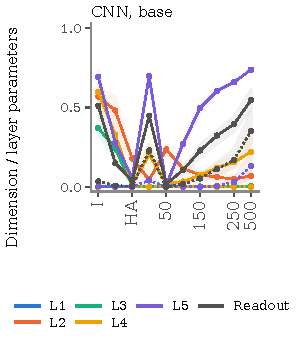
\includegraphics[width=1.804in]{compact_tails_part2.pdf}
\caption{Continued. Approximate atomic dimensions for models measured at multiple training stages, with all measured layers shown. MNIST is used unless labeled SVHN; layer numbers refer to hidden layers or convolutional layers. Solid curves count singular values at most $10^{-3}\sigma_1$ and dotted curves use $10^{-9}\sigma_1$, each divided by layer parameter count. Lines are seed means and bands are seed ranges. Missing measurements remain gaps. Stage positions are categorical, with abbreviations as in the atomic panels.}

\end{figure}
\FloatBarrier
